% % % % % % % % % % % % % % % % % % % % % % % % % % % % % % % % % % % % % % % %
% LaTeX4EI Example for Cheat Sheets
%
% @encode: 	UTF-8, tabwidth = 4, newline = LF
% @author:	LaTeX4EI
% % % % % % % % % % % % % % % % % % % % % % % % % % % % % % % % % % % % % % % %


% ======================================================================
% Document Settings
% ======================================================================

% possible options: color/nocolor, english/german, threecolumn
% default: color, english
\documentclass[english]{latex4ei/latex4ei_sheet}

% set document information
\title{SoC Cheat Sheet}
\author{Fabian Olbert}					% optional, delete if unchanged
\myemail{fabian.olbert@gmail.com}			% optional, delete if unchanged


% DOCUMENT_BEGIN ===============================================================
\begin{document}

\maketitle	% requires ./img/Logo.pdf

\section{Introduction}

\textbf{Moores Law}: The number of transistors per chip will continue to double every 18 – 24 months.

\subsection{MOSFET}
\textbf{off}: \qquad $I_{Dn} = 0$ \qquad $V_{GS} < V_t \wedge V_{DS} \geq 0$

\textbf{linear}: \qquad $I_{Dn} = \beta (V_{GS} - V_t - \frac{V_{DS}}{2})V_{DS} $ \qquad $V_{GS} > V_t \wedge  0 < V_{DS} < V_{GS} - V_t$

\textbf{saturation}: \qquad $I_{Dn} = \frac{\beta}{2} (V{GS} - V_t)^2$ \qquad $V_{GS} > V_t \wedge  V_{DS} > V_{GS} - V_t$

\subsection{Effect of Capacitance on Inverter Delay}
$t_{pHL} \varpropto \frac{C_{load} t_{ox} L_p}{W_p \mu_p \epsilon_{Ox} (V_{DD} - |V_{tp}|)}$

$t_{pHL} \varpropto \frac{L_p}{W_p \mu}$

\subsection{CMOS Power}
\textbf{Dynamic Capacitive Power}: $P_{cap} = \alpha_{01} f C V_{dd}^2$

\textbf{Short Circuit Power}: $P_{short} = \alpha_{01} f \beta_n \tau (V_{dd} - 2 V_{tn})^3$

\textbf{Sub Threshold Currents}: $I_D = I_0 e^{(V_{GS} - V_t) / n V_{temp}} (1 - e^{-V_{DS} / V_{temp}}$

\textbf{Diode Leakage Gate current}:

%\begin{center}
%    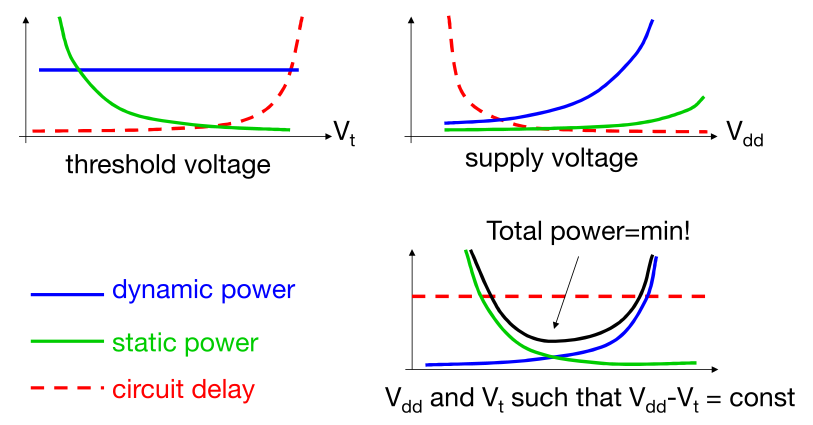
\includegraphics[width = 5cm ]{images/1. Introduction/power_curve.png}
%end{center}


\section{SoC Logic Design Recap}
\textbf{AND}: $A B$
\textbf{NAND}: $\overline{A B}$
\textbf{OR}: $A + B$
\textbf{NOR}: $\overline{A + B}$
\begin{center}
	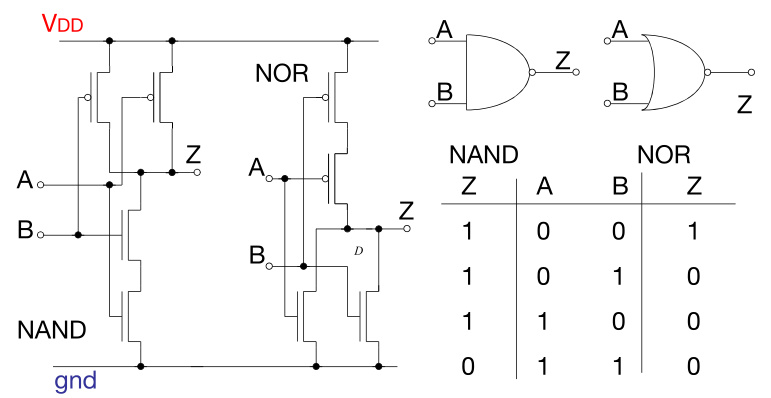
\includegraphics[width = 5cm ]{images/2. SoC Logic Design Recap/NandNor.png}
\end{center}
\subsection{DeMorgan}
\begin{center}
	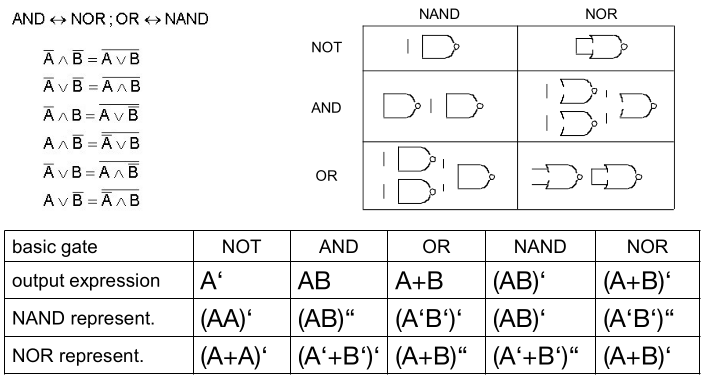
\includegraphics[width = 5cm ]{images/2. SoC Logic Design Recap/DeMorgan.png}
\end{center}
\subsection{Static CMOS Logic Design}
\begin{enumerate}
	\item[$\bullet$] CMOS always inverts $Z = not(not(A + C))$
	\item[$\bullet$] Start at the output and find a way through n-MOSFETS to ground: (serial for AND (AB) , parallel for OR (C)
	\item[$\bullet$] Draw the way to Vdd by using the dual n-network and p-MOSFETS
	\item[$\bullet$] \textbf{If everything is done right, there will
		      never be a conducting path between Vdd
		      and gnd.}
\end{enumerate}



\subsection{Flip Flop Timing}

\textbf{setup-time}: Data must be stable $t_{setup}$ before the clock edge

\textbf{hold-time}: Data must be stable $t_{hold}$ after the clock edge

\textbf{clock-to-output-delay}: Data will be visible at output after $t_{c2q}$ after clock edge

\textbf{Setup constrain} $T_{clk} > T_{c2q} + T_{logic, max} + T_{setup}$

\textbf{Hold constrain} $T_{c2q} + T_{logic, min} > T_{hold}$

\textbf{Metastability}: Violation of either setup-time or hold-time restrictions may result in undefined or oscillating output signals of a flip-flop.


\subsection{Finite State Machines}

\textbf{Moore Machine} Output Z only dependent on current state $S_i$

\textbf{Mealy Machine} Output Z dependent on current state $S_i$ and input A

\begin{center}
	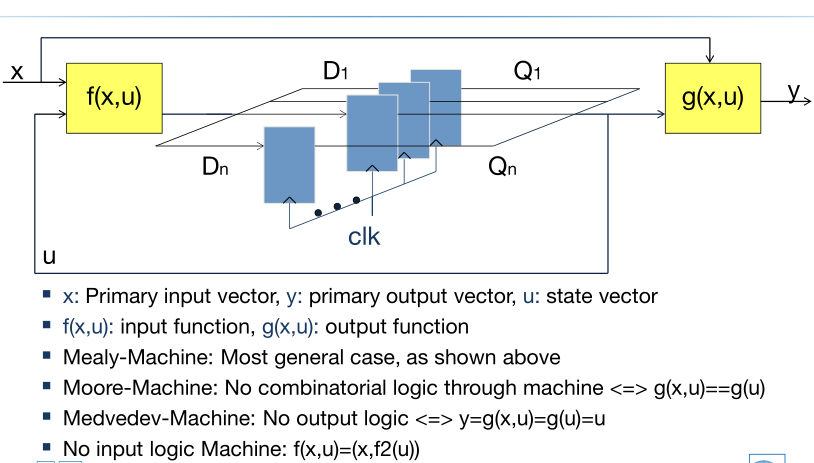
\includegraphics[width = 5cm]{images/2. SoC Logic Design Recap/FSM.png}
\end{center}
\begin{center}
	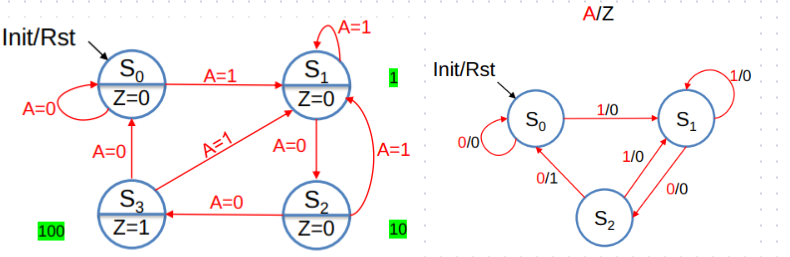
\includegraphics[width = 5cm]{images/2. SoC Logic Design Recap/MooreMealy.png}
\end{center}

\textbf{FSM Logic Depth}: $N = \frac{T_{clk} - T{setup} - T_{c2q}}{t_{gate} + t_{wire}}$



\section{SoC Paradigm}
\begin{center}
	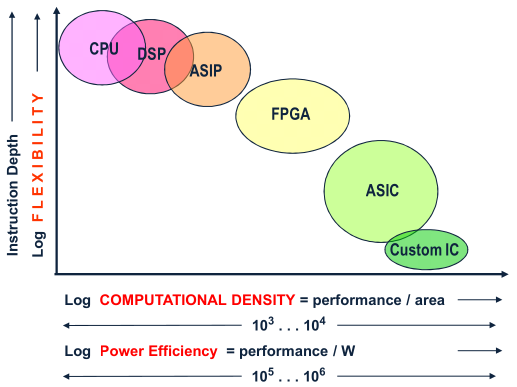
\includegraphics[width = 5cm]{images/3.SoCParadigm/Paradigm.png}
\end{center}

\textbf{Revisiting Moores Law} Designers productivity does not scale equal to chip capacity $>$ Design Teams are growing to keep constant dev time

\textbf{Platform-based SoC Design}: SoC is an integrated system design paradigm where large portions of a chip are assembled from already existing function blocks maintained in so called Core or Macro Libraries.

\textbf{Virtual Platforms}: To reduce the overall design time, the software development can start much earlier on a virtual platform (VP). A VP is an accurate model of the system hardware.

\textbf{Trade-Off: Flexibility vs. Performance} maybe insert image

\textbf{Computational density} (CD) is defined as computations per unit area and time.
$CD = \frac{computational\_power}{area}$ where $area = \frac{siliconarea [nm^2]}{\lambda^2 [\mu m^2]}$ and $computational\_power = Data size * IPC * frequency$

\begin{enumerate}
	\item CPU: 40 - 80
	\item FPGA: 400
	\item Asic 4000
	\item Custom  $>$ 10000
\end{enumerate}

The actual computational power is lower because of Memory Latency, Pipeline Stalls, Cache Misses, Instruction Dependencies, Branch Prediction Failures

For FPGAs and Asics we have a standard activity factor $\alpha$ of 0.2 and 0.1 since not every LUT/logic is used for every clock cycle. (Multiply computational power by nLUTs for MAX CD)

$[CD] = \frac{ops}{N [L_{min}^2 tiles]} = \frac{1 operation}{s \cdot sq}
	= \frac{1M operations}{1s \cdot mm^2 / \mu m^2}$

\textbf{Functional Diversity} (FD) Number of functions resident and rapidly accessible by a compute unit

\begin{enumerate}
	\item CPU: 256K - 16K
	\item FPGA: 1
	\item Asic $10^{-3}  - 10^{-6}$
	\item Custom  $\approx$ 0
\end{enumerate}

\textbf{Software vs. Hardware Implementation}The fundamental difference between HW and SW implementation is the degree of parallelism that can be achieved during the execution of the target functionality. Parallel in space, sequential in time vs parallel in space and time

\textbf{Gate Array}Gate Array architecture consists of an array of prefabricated transistors. These transistors are supplied with VDD and GND connections (lower left hand figure on the slide). Any circuit can be implemented using these transistors by depositing wire interconnects on top of the array.

\textbf{Standard Cell}In a Standard Cell ASIC there are no prefabricated transistors, but a library of pre-developed logic cells instead. Any circuit can be implemented using these cells.

\textbf{Asic}

\textbf{Full Custom Design}
In a Full Custom design, individual transistors, logic gate cells and coarse grain function macros are placed unconstraint (with respect to placement grids) and optimized individually resulting in minimum area and power at maximum performance.

\textbf{Programmable Logic Devices (PLD)}
In contrast to ASIC chips or Full Custom Design, the functionality of programmable logic can be modified after chip fabrication.
Programmable Array Logic (PAL) and Programmable Logic Array (PLA). PAL is composed of programmable AND matrix and OR matrix, while in PLA the OR matrix is fixed.

\textbf{FPGA}
The basic ingredients of an FPGA are configurable logic blocks (CLBs), configurable routing resources and I/O pads. Each CLB contains multiple look-up tables which are configured by the program data.

\begin{center}
  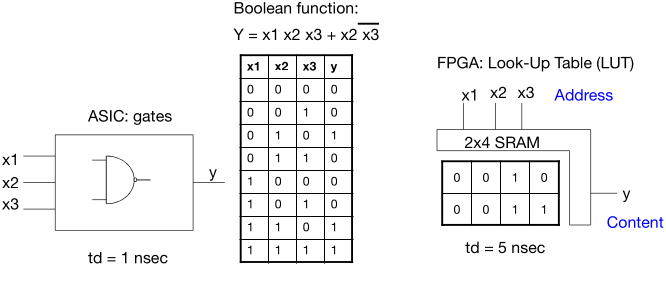
\includegraphics[width=\linewidth]{assets/FPGARealization.png}
  \label{fig:fpgarealization}
\end{center}

The content of the lookup table is the result y and the address is equivalent to the input x1 \& x2 \& x3.

\textbf{single vs. multicore}:
$P_{dyn} = f V_{dd}^2 N $\quad N: number cores

Assumption: App can be perfectly parallelized on n cores:

Case 1: Single- and Multi-core have same execution time $T_{exe}$

$P_{dyn} \sim \frac{f V_{dd}^2}{n^2}$

Case 2: Multi-core shall have performance increase by factor k

$P_{dyn} \sim \frac{k^3 f V_{dd}^2}{n^2}$

$power\_savings = \frac{P_{dyn, after}}{P_{dyn, before}}$

\section{Processor Architecture}

A program is executed in the following sequence:
\begin{enumerate}
	\item[$\bullet$] \textbf{Instruction Fetch (IF)}
	\item[$\bullet$] \textbf{Instruction decode (ID)}
	\item[$\bullet$] \textbf{Execution (EX)}
	\item[$\bullet$] \textbf{Memory (MEM)}
	\item[$\bullet$] \textbf{Write back (WB)}
\end{enumerate}

\textbf{Instruction Level Pipelining}
\begin{center}
	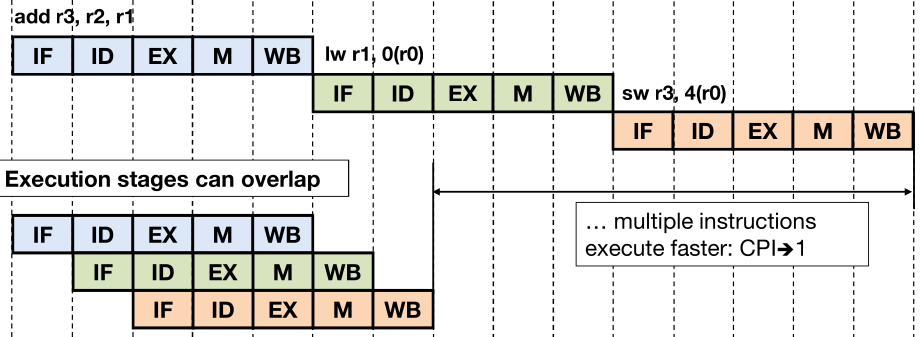
\includegraphics[width = 5cm]{images/4.ProcessorArchitecture/ILP.png}
\end{center}

\textbf{CPU Pipeline} Maximum Clock frequency is determined by longest path: $f_{max} = \frac{1}{T_{clk}}$

\textbf{Structural Hazards} Structural hazard occur if a resource conflict exists between instructions in the pipeline.
\begin{center}
	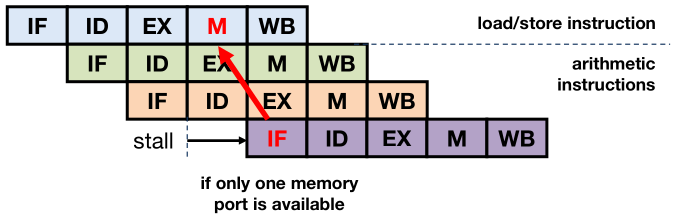
\includegraphics[width = 5cm]{images/4.ProcessorArchitecture/StrHazard.png}
\end{center}

\textbf{Data Hazards} In a pipeline, a data hazard arises if a result of an operation is required before it has been calculated. (stalling is required)
\begin{center}
	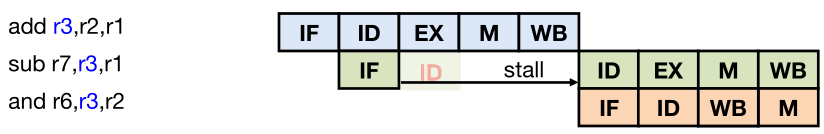
\includegraphics[width = 5cm]{images/4.ProcessorArchitecture/DataHazard.png}
\end{center}

\textbf{Control Hazards} Deviations from the sequential execution of a program may result in pipeline problems as
well. If a branch operation causes the program counter to jump to another location, the instructions in the pipeline following the branch has to be flushed and the pipeline has to be filled again starting from the correct instruction.
\begin{center}
	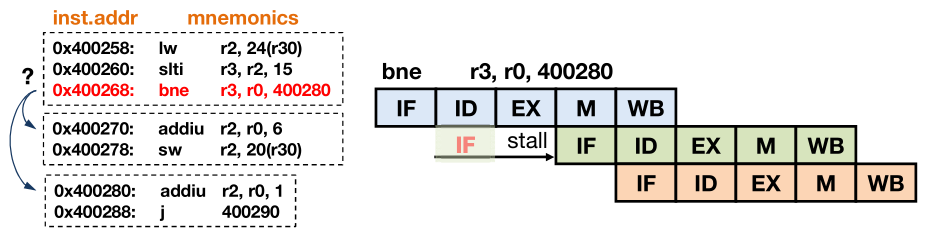
\includegraphics[width = 5cm]{images/4.ProcessorArchitecture/ControlHazard.png}
\end{center}

\textbf{Register Forwarding}
Execute after Execute instructions and after Memory Access for load instructions:
\begin{center}
	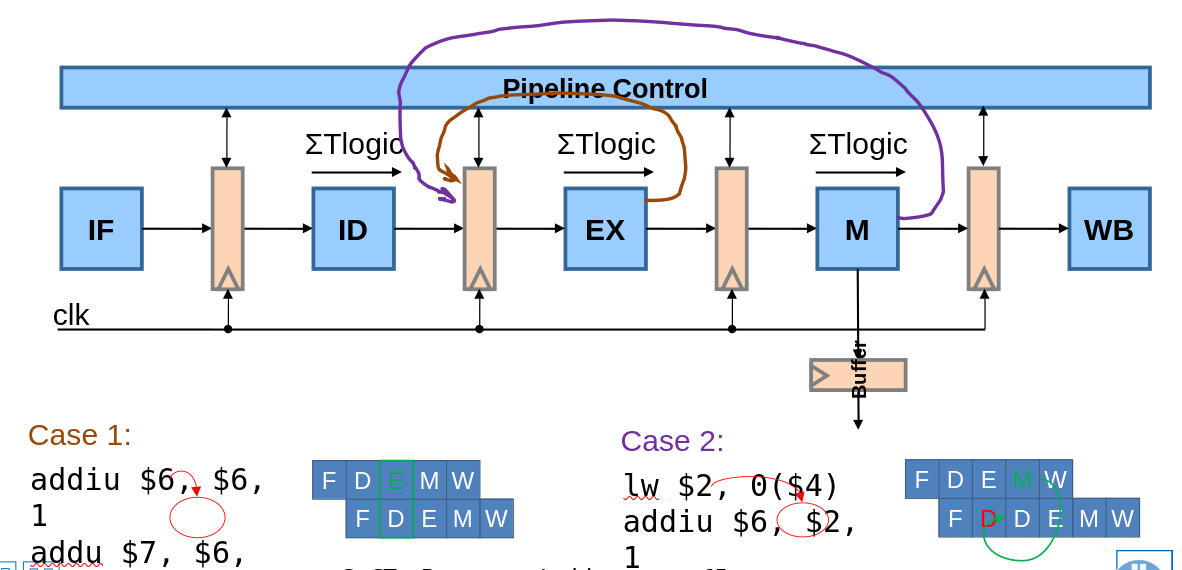
\includegraphics[width = 5cm]{images/4.ProcessorArchitecture/RegisterForwarding.png}
\end{center}

\textbf{Branch Prediction} Reduces the impact of control hazards in the pipeline. In a 1-bit branch predictor, the last outcome of a branch (taken or not taken) is stored in a 1-bit branch history table. The table is indexed by last x bits of the branch address, and, thus, the branch table contains $2^x$ elements in total.
\begin{center}
	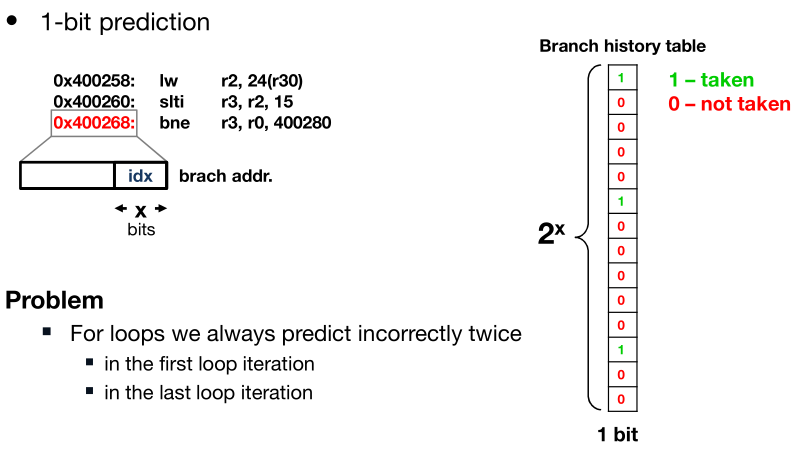
\includegraphics[width = 5cm]{images/4.ProcessorArchitecture/1BitPred.png}
\end{center}

\begin{center}
	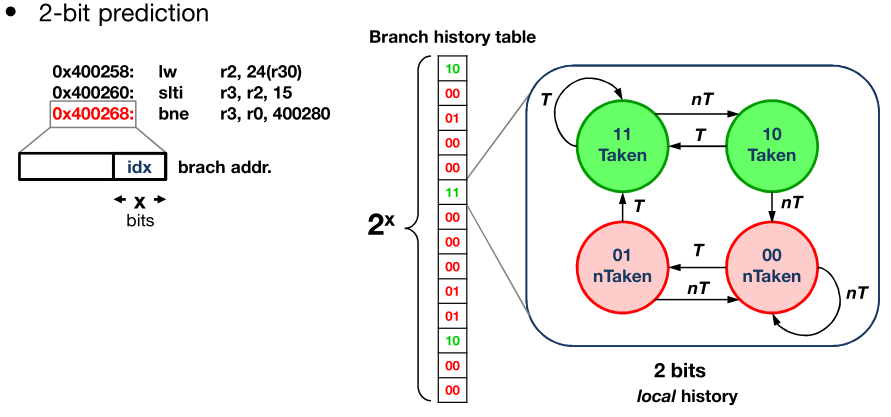
\includegraphics[width = 5cm]{images/4.ProcessorArchitecture/2BitPred.png}
\end{center}



\textbf{ILP: Superscalar Architecture} To exploit ILP even further, superscalar processors contain multiple execution units, and multiple instructions can be executed in parallel as long as there are no dependencies among them. CPI $<$ 1 possible, scheduled during runtime

\textbf{ILP: VLIW processors} scheduled during compile time

\textbf{Processor Performance} $CPU_{time} = \frac{Inst}{Prog} \frac{clk\_cyc}{Inst} \frac{Seconds}{clk\_cyc}$

CPI: Cycles per Instruction

$CPI = CPI_{cpu} + CPI_{mem}$

$CPI_{mem} = CPI_{inst} + CPI_{data}
	\newline = I_{freq} \cdot L1_{miss\_rate} (L1_{miss\_penalty} + L2_{miss\_rate} \cdot L2_{miss\_penalty}) + D_{freq} \cdot L1_{miss\_rate} (L1_{miss\_penalty} + L2_{miss\_rate} \cdot L2_{miss\_penalty})$

\textbf{Cache Organization}

\begin{center}
	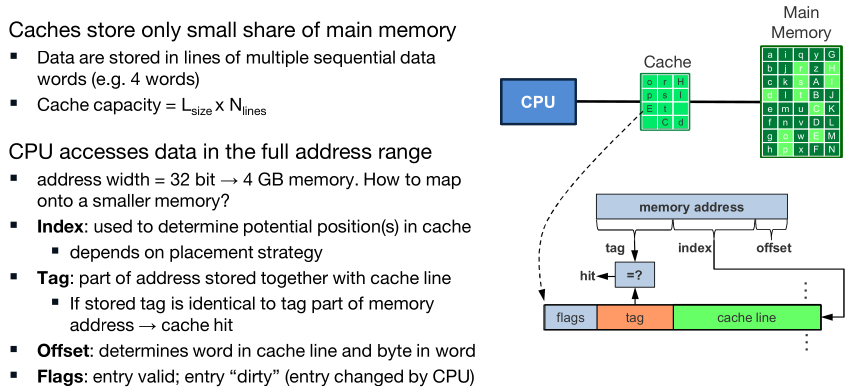
\includegraphics[width = \linewidth]{images/4.ProcessorArchitecture/cache.png}
\end{center}

$\#cache\_lines = \frac{cache\_size}{line\_size \cdot \#of\_ways}$

$Index = log_2(\#cache lines)$

$Offset = log_2(Cache line size)$

$Tag = Address_{size} - Offset - Index$

\textbf{Set Associative Cache}
Can improve performance whe the processor frequently accesses different memory addresses with identical index.
\begin{center}
	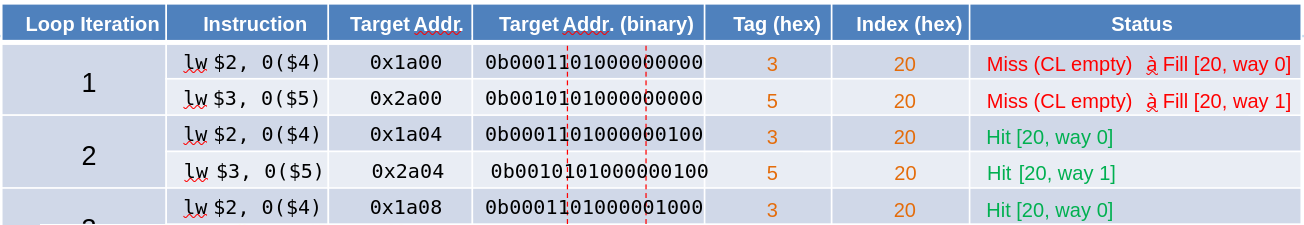
\includegraphics[width = 6cm]{images/4.ProcessorArchitecture/SetAcCache.png}
\end{center}

\textbf{Cache Replacement}
If all entries are occupied by an entry now, one of them needs to be evicted. The decision on which entry to replace is defined by a replacement policy that is optimized in a way that the number of misses is reduced.

\textbf{Cache Write Strategies}

\begin{center}
  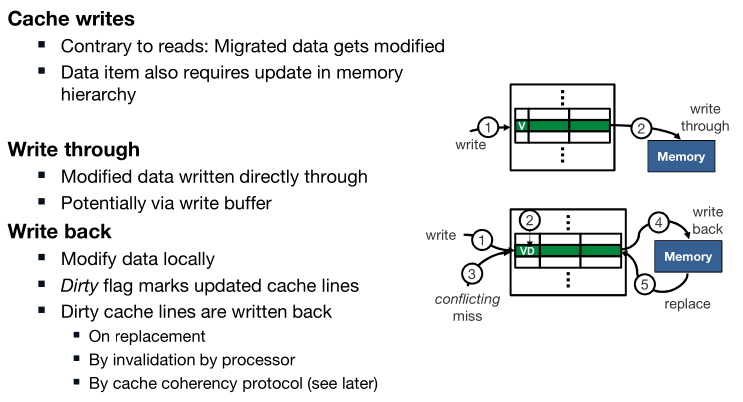
\includegraphics[width=\linewidth]{assets/CacheWriteStrategies.png}
  \label{fig:cachewritestrategies}
\end{center}

\textbf{Multithreading in Software}

\textbf{Multithreading in Hardware}



\textbf{Memory Hierarchy}

\begin{center}
	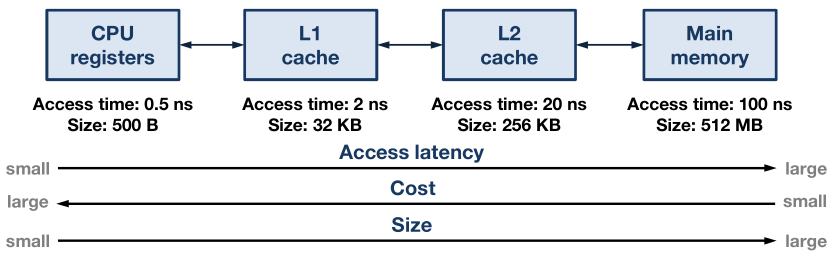
\includegraphics[width = 5cm]{images/4.ProcessorArchitecture/MemoryHierarchy.png}
\end{center}

Temporal locality: addresses are likely to be accessed in the near future once again

Spatial locality: addresses are likely to be close to each other

\section{Memory}
\begin{center}
	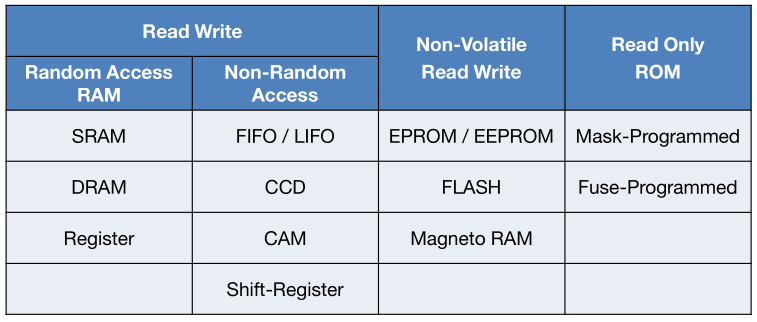
\includegraphics[width=5cm]{images/5.Memory/MemoryClassificatoin.png}
\end{center}
\begin{center}
	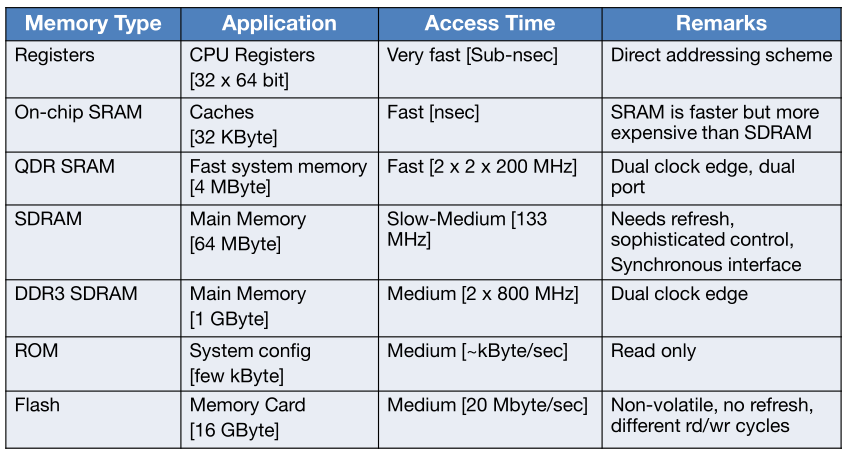
\includegraphics[width=5cm]{images/5.Memory/MemoryCharacteristics.png}
\end{center}

\textbf{Bandwith}: Amount of data transported into or out of a memory array (or
memory interface) per unit of time.

\textbf{Latency}: Delay or time elapsed between the request and actual delivery of data.

\textbf{Cycle time}: Minimum time period between two consecutive read or write accesses
to memory.

\textbf{Asynchronous memory vs Synchronous memory} hanging address or
control signal lines trigger the reading or writing of data vs synchronous to clock signal.

\textbf{Decoders} reduces \# of select signals to $K = log_2 N$

\textbf{Array Structure} The address decoder is split into a column decoder, which selects one out of 2 K words from a word line, and a row decoder, which selects one out of 2L-K word lines. Allows Burst mode.
\begin{figure}
	\centering
	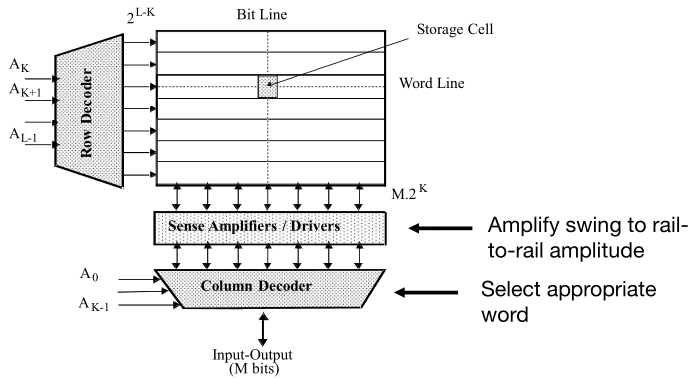
\includegraphics[width=1\linewidth]{images//5.Memory/ArrayStructure.png}
\end{figure}

\textbf{Hierarchical Memory Architecture}

\textbf{DRAM} requires minimum amount of CMOS transistors

$Q = C V$

$\Delta V = V_{BL} - V{PRE} = (V_{Bit} - V_{PRE})\frac{C_S}{C_S + C_{BL}}$

where $V{Bit}$ : (0V, $V_{dd}$) and $V_{PRE} = \frac{V_{dd}}{2}$

\begin{figure}
	\centering
	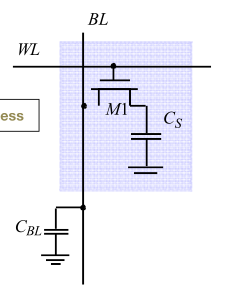
\includegraphics[width=1\linewidth]{images//5.Memory/DRAMCell.png}
\end{figure}

\textbf{Trench DRAM Cell} use Trench in substrate to create capacitor.

\textbf{Sense Amplifier} Voltage swing in DRAM capacitor is a lot less than $V_{dd} / 2$ therefore Amplifier is required to be either 0 or $V_{dd}$... also accelerates towards 0 or $V_{dd}$

\textbf{T-Transistor SRAM Cell}

\textbf{SRAM} Stable Feedback Loop, no capacitor needed, more space than SDRAM

\textbf{ROM} mask programmable, one time programmable(fuses), BIOS (boot code)

\textbf{DDR} Double data SDRAM allows for transfering data words on rising and falling edge. DDR3 SDRAM has higher clock frequencies.

\textbf{SDRAM Read Operation Timing}

$nCycles = latency + nWords_{Burst} + t_{newRowAddr}$ \quad only one cycle

$rate = \frac{bytes * f}{nCycles}$

\textit{Best Case}: all words have the same row address

\textit{Worst Case}: all words have different row addresses

\textbf{SDRAM Write Operation Timing}
1. Decoding row address 2. activation of the row 3. decoding of the column address 4. selection of a column entry and transfer to output buffer
\begin{center}
	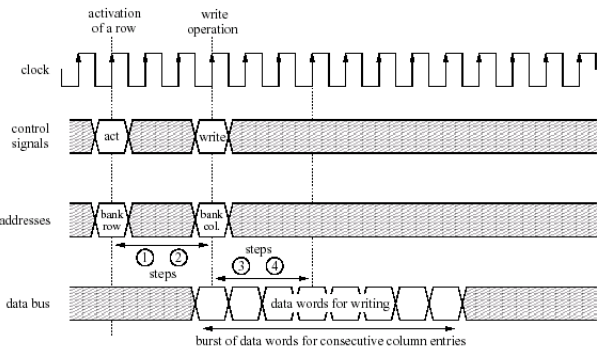
\includegraphics[width=5cm]{images//5.Memory/SDRAMWrite.png}
\end{center}

\section{Interconnect}

\textbf{On-Chip Buses}
\begin{center}
	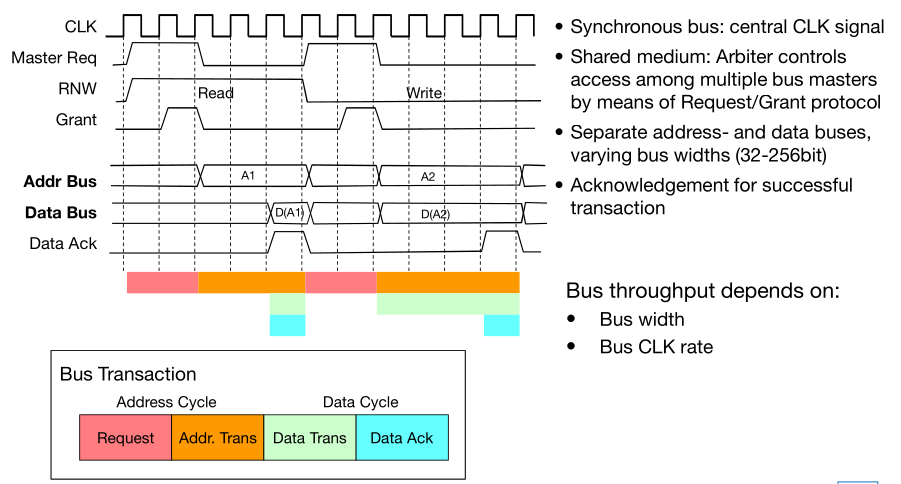
\includegraphics[width=\linewidth]{images//6.Interconnects/OnChipBasicOperation.png}
\end{center}
Bus throughput depends on \textbf{Bus width} and \textbf{Bus CLK rate}

\paragraph{Bus Arbitration Schemes} Determine sequence in which requests from multiple masters are serviced
\begin{figure}
	\centering
	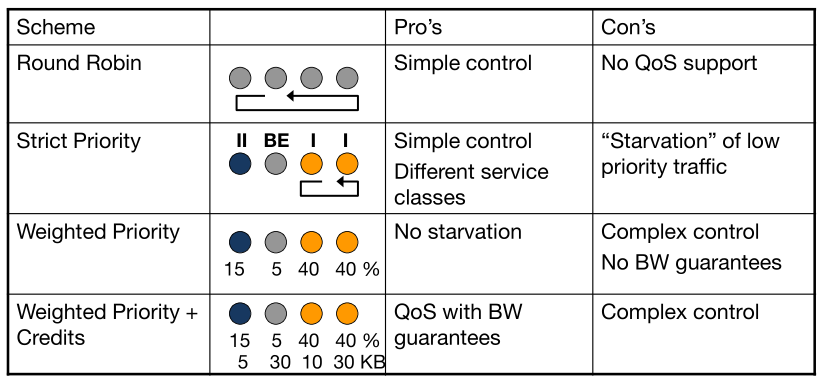
\includegraphics[width=\linewidth]{images//6.Interconnects/BusArbitrationSchemes.png}
\end{figure}

\paragraph{PLB(Processor Local Bus)}

\begin{center}
	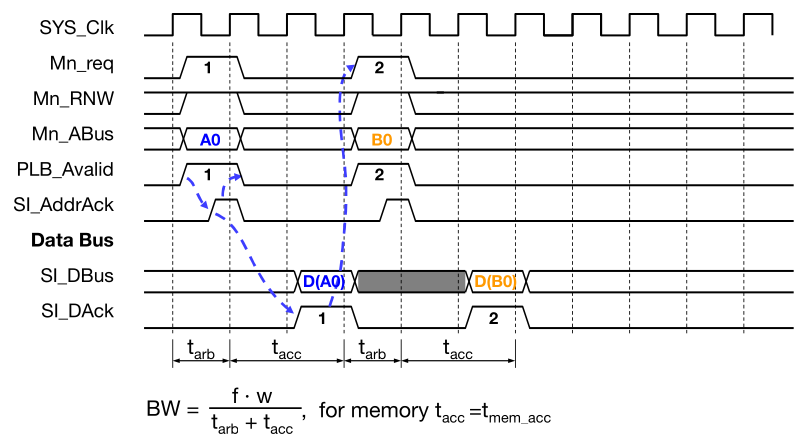
\includegraphics[width=\linewidth]{images//6.Interconnects/PLBTiming.png}
\end{center}

\paragraph{Bus Imporovements}
\begin{enumerate}
	\item Independent data buses for reads writes
	\item Pipelining
	\item Burst Transfers
\end{enumerate}

\paragraph{Pipelined Bus Control}
\begin{center}
	\centering
	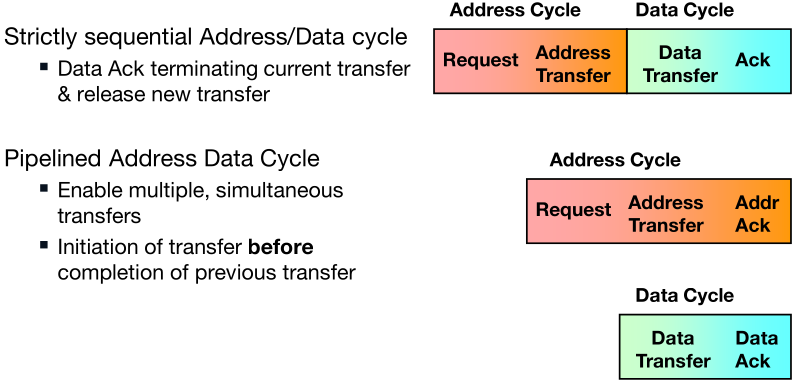
\includegraphics[width=0.75\linewidth]{images//6.Interconnects/PipelinedBusControl.png}
\end{center}

\paragraph{Burst Transfers} Reduction of Req./Addr. signaling overhead for read/write transactions to consecutive addresses.

$BW = \frac{f \cdot w \cdot n}{(t_{arb} + t_{acc}) + (n - 1)}$
\paragraph{Pipelined Burst Rd Transfers}

$BW = \frac{f w n}{n} = f \cdot w$

\paragraph{Pipelined Back-to-Back Rd \& Wr}

\paragraph{AMBA AHB} AHB employs a bus arbiter for deciding which master can be granted
access to the bus and contains independent read data buses for write data buses. In addi-
tion, AHB is capable of pipelined and burst transfers. An interesting feature of AHB is split
transfers.

\paragraph{AMBA AXI} Out-of-order transfers

\paragraph{Bus Standards Comparison}
\begin{center}
	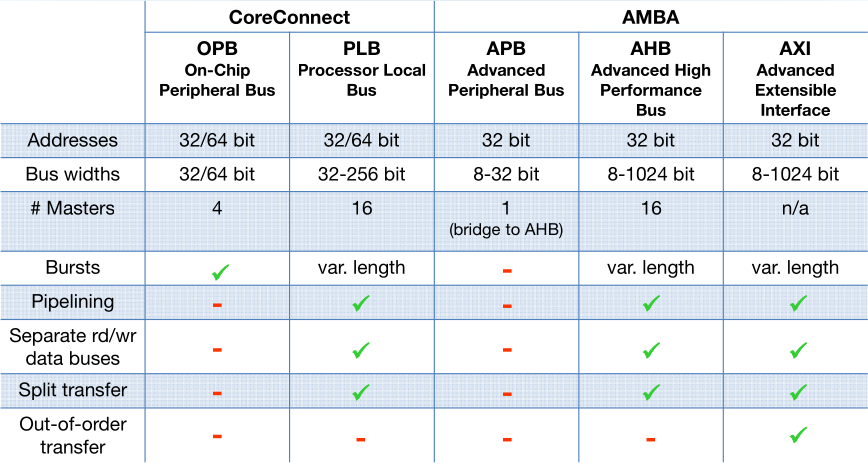
\includegraphics[width=0.75\linewidth]{images//6.Interconnects/BusComparison.png}
\end{center}


\paragraph{FIFO}

\textit{FIFO used for}:
\begin{enumerate}
	\item Decoupling clock domains
	\item Decoupling data path widths
\end{enumerate}
\textit{FIFO size}:
\begin{enumerate}
	\item as small as possible
	\item large enough to compensate for different read/write data rates
\end{enumerate}
\begin{center}
	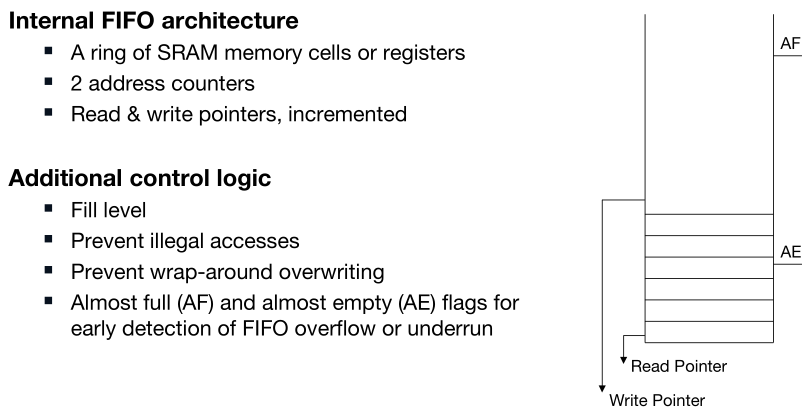
\includegraphics[width=0.75\linewidth]{images//6.Interconnects/FIFO.png}
\end{center}

\textbf{Basic Packet Rx} On-chip bus communication demand can be magnitude higher than the aggregate line rate.
\textit{Improvements}
\begin{enumerate}
	\item Multiple, physical memories
	\item Separation data, state, control
	\item Interleaving techniques
	\item Multi-port memories
\end{enumerate}

\paragraph{Noc - Network on Chip}
\textit{Benefits}
\begin{enumerate}
	\item Scalablity
	\item Segmentation of wires: short point-to-point links
	\item Synchronization
\end{enumerate}
\textit{Drawbacks}
\begin{enumerate}
	\item Latency
\end{enumerate}

\section{Questions}

\begin{enumerate}
	\item The functionality of programmable logic inside the FPGA can be modified after chip fabrication
	\item In a write through cache policy, a dirty flag is not required to mark the changed line
	\item For loops, a two-bit branch predictor performs worse than a one-bit predictor in the first iteration

\end{enumerate}

\section{to do}
\begin{enumerate}
	\item in a system bus how can i detect the difference between read write
	\item add cpi formula
\end{enumerate}




\end{document}
